%replace the figure labelled "albedo_grain" with the following:

\begin{figure*}
\begin{center}
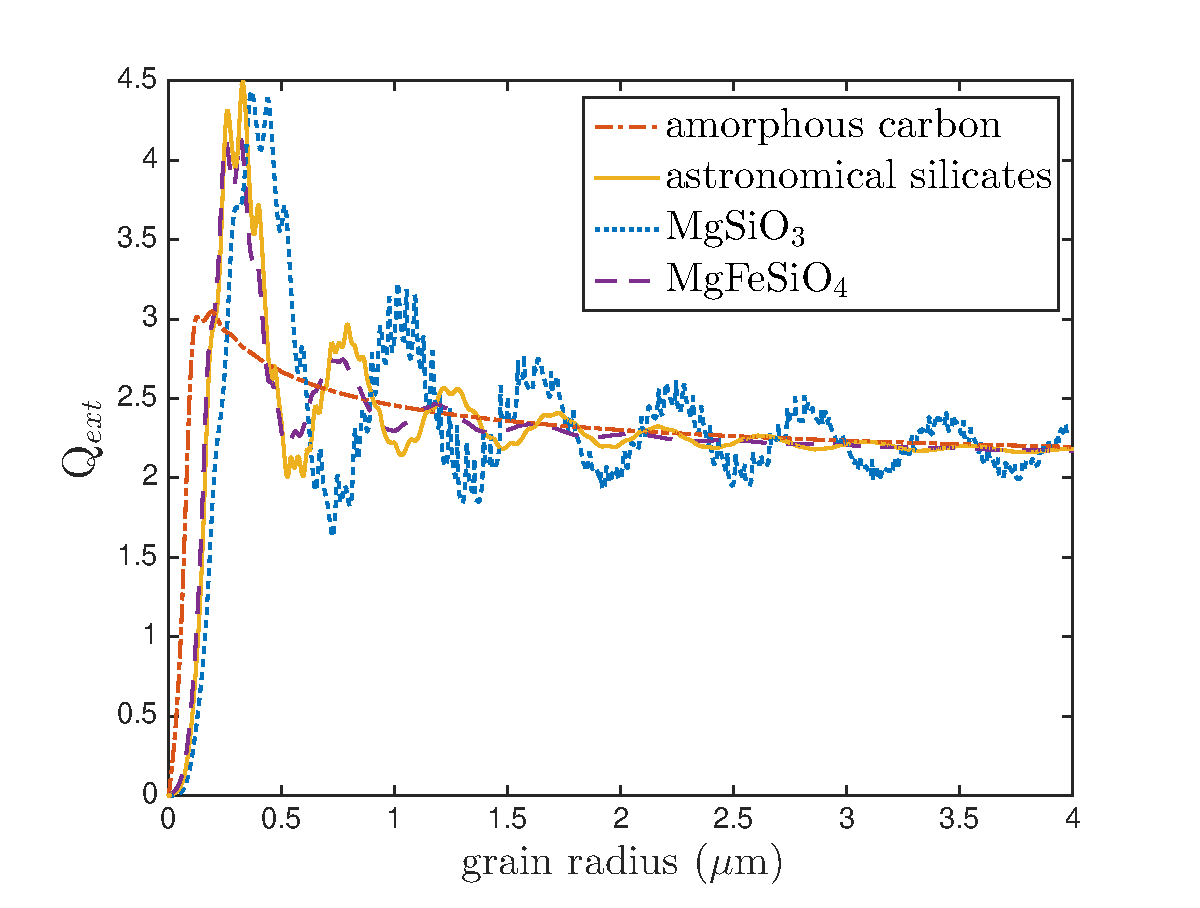
\includegraphics[trim =37 10 45 15,clip=true,scale=0.51]{Qext_grainsize_upto4}
\includegraphics[trim =37 10 45 15,clip=true,scale=0.51]{Qext_grainsize_upto4_log}
\includegraphics[trim =37 10 45 15,clip=true,scale=0.51]{albedo_grainsize_upto4}
\includegraphics[trim =37 10 45 15,clip=true,scale=0.51]{albedo_grainsize_upto4_log}
\caption{Variation of albedo and extinction efficiency ($Q_{ext}$) with grain size for amorphous carbon and silicates sample using a Mie approximation at $\lambda = 658 \mu $m. Optical constants from \citet{Zubko1996} and \citet{Draine1984}. A linear scale is presented on the left and a log scale on the right.}
\label{albedo_grain}
\end{center}
\end{figure*}


%I envisage this going below the subsection on the clumped models and above the subsection entitled "Contamination of the the H$\alpha$ profiles at days 704 and 806".

\subsection{The effect of a grain size distribution}
\label{gs_distn}
It is important to consider the potential effect on the dust mass of modelling a grain size distribution instead of a single grain size.  For a grain size distribution the overall extinction cross section, $C_{ext}$, at a given wavelength is calculated as

\[ C_{ext}=\int^{a_{max}}_{a_{min}} Q_{ext}(a) n(a) \pi a^2 da \]

where $Q_{ext}(a)$ is the extinction efficiency for a grain size $a$ and $n(a)$ is the number of grains with size $a$. The overall extinction efficiency is then

\[ Q_{ext} = \frac{C_{ext}}{ \int^{a_{max}}_{a_{min}} n(a) \pi a^2 da} \]
 
The scattering cross-section $Q_{sca}$ is similarly calculated.  As a result of these calculations, there is rarely a single grain size that has the same albedo and extinction efficiency as a size distribution.  Modelling a size distribution may therefore alter the deduced dust mass.  Since the models are only sensitive to the optical depth and the albedo, however, it is not possible to deduce the grain size range or distribution and only single grain sizes are investigated (as presented above).

Whilst this apparently limits the scope of the results, it is important to consider the extent to which considering grain size distributions would alter the derived dust masses.  By considering a number of grain size ranges and adopting a power law distribution with a variable exponent, we may gain some insight into the effects of adopting a distribution rather than a single size.  For the classical MRN power law ($n(a) \propto a^{-3.5}$) with a wide grain size range ($a_{min} = 0.001 \mu$m to $a_{max} = 4.0 \mu$m) the derived albedo is much too small to reproduce the required wing seen at early epochs.  We therefore adopt an approach whereby, for a number of grain size ranges, we adjust the exponent of the distribution until the overall albedo is the same as that seen for the best fitting single grain size for the clumped distributions.  We may then approximately calculate the required dust mass as

\begin{equation}
\label{distn_conv}
M_{d}= \frac{M_s Q_{ext,s}(a_s)}{a_s} \times \frac{\int^{a_{max}}_{a_{min}} n(a) a^3 da}{\int^{a_{max}}_{a_{min}} Q_{ext}(a) n(a) a^2 da}
\end{equation}

where the subscript $s$ represents the single grain size quantities and the $d$ subscript represents quantities for the grain size distribution.  

We calculate the required dust masses for the clumped model on day 714 for a selection of distributions with varied $a_{min}$.  These are presented in table \ref{tb_distn}.  It can be seen that in all cases, a larger dust mass is required in order to reproduce the same conditions as a single grain size.  The conversion factors presented in the table are valid for any model with grain size $a=0.6\mu$m and may therefore also be applied to the models for day 806.  We repeated the process for $a=3.5 \mu$m but found that, in order to reproduce the required albedo, the distribution had to be heavily weighted towards the larger grains and that the value of $a_{min}$ had no effect of the required dust mass.  Increasing the value of $a_{min}$ to larger values (>2$\mu$m) does not have a significant effect either.  This is because both extinction efficiency and albedo tend to a constant value with increasing grain radius and the adoption of different grain size ranges and distributions above a certain threshold therefore results in only insignificant variation in these quantities. 

\begin{table}
	%\begin{minipage}{180mm}
	\caption{Equivalent dust masses for the day 714 clumped models using grain size distributions and 100\% amorphous carbon. $f$ is factor of increase from the dust mass for the single size model ($M=7 \times 10^{-5} M_{\odot}$ with $a=0.6 \mu$m) and $p$ is the exponent of the grain size distribution $n(a) \propto a^{-p}$.}
	\label{tb_distn}
	\begin{center}
  	\begin{tabular}{@{} ccccc @{}}
    	\hline
$a_{min}$ & $a_{max}$ & $p$ & $M$ & $f$  \\%& $Q_{ext}$ \\
($\mu$m) & ($\mu$m) & & ($M_{\odot}$) & \\
\hline
0.001 & 4 & 2.45 & 1.93E-04 & 2.76 \\%& 2.13 \\
0.01 & 4 & 2.45 & 1.93E-04 & 2.76 \\%& 2.32 \\
0.05 & 4 & 2.52 & 1.84E-04 & 2.62 \\%& 2.44 \\
0.1 & 4 & 2.72 & 1.61E-04 & 2.3\\ %& 2.53 \\
0.5 & 4 & 8.2 & 7.23E-04 & 1.03 \\%& 2.61 \\

    \hline
  \end{tabular}
  \end{center}
%\end{minipage}
\end{table}

This calculation in equation \ref{distn_conv} holds only for a single wavelength and therefore is not exact for our models which obviously transport radiation over a range of wavelengths.  However, the dust masses derived using the above formula produce almost identical fits to the data as for the single grain size and therefore give an excellent suggestion of the approximate dust mass required when using a distribution.

We therefore conclude that, if a distribution of grain sizes is indeed present, the deduced dust masses are likely to be under-estimating the true mass of newly formed dust rather than overestimating it.

\subsection{The effect of different species}

In all of our analyses heretofore, we have considered only amorphous carbon as the species of interest.  This is in part motivated by previously published literature that suggests that, if silicates do form a fraction of the total dust mass, it is likely that that fraction is limited to approximately 15\% (W15, \citet{Ercolano2007}).  It is also partly motivated by the nature of the model; the parameters that affect the quantity of dust required in the model are the albedo and the optical depth.  There are likely many possible combinations of species and grain sizes that result in a good fit to the data.  

We consider the change in dust mass when a medium of 100\% silicates is used instead of amorphous carbon.  We use optical constants presented in \cite{Draine1984}.  In a similar manner to the approach detailed in section \ref{gs_distn}, we may calculate the mass of silicates that is equivalent to a carbon mass for a single grain size.  We consider the albedo at the original grain size, calculate the equivalent grain size for silicates that results in the same albedo and then calculate the new dust mass by considering the change in the extinction efficiency as

\begin{equation}
M_{sil} = M_{amc} \Big( \frac{Q_{amc}}{Q_{sil}} \Big) \Big(\frac{a_{sil}}{a_{amc}}\Big) \Big(\frac{\rho_{sil}}{\rho_{amC}}\Big)
\end{equation}

Because of the nature of the variation of albedo with grain size for silicates (see figure \ref{albedo_grain}), there is often more than one silicate grain size that will give rise to the same albedo.  We consider all the possibilities and the resulting mass conversion factors in table \ref{tb_sil}.  In our best fitting models for days 714 and 806, using any fraction of silicates of either grain size would serve to increase the dust mass.  However, at later epochs, using some fraction of silicate dust would reduce the dust mass to potentially more than half of our estimated values. However, this is still within our predicted range and our minimum and maximum dust masses remain robust.

\begin{table}
	%\begin{minipage}{180mm}
	\caption{Equivalent dust masses for the day 714 clumped models using grain size distributions and 100\% amorphous carbon. $f$ is factor of increase from the dust mass for the single size model ($M=7 \times 10^{-5} M_{\odot}$ with $a=0.6 \mu$m) and $p$ is the exponent of the grain size distribution $n(a) \propto a^{-p}$.}
	\label{tb_sil}
	\begin{center}
  	\begin{tabular}{@{} cccccc @{}}
    	\hline
	\multicolumn{2}{c}{\textit{carbon}} && \multicolumn{2}{c}{\textit{silicates}} & \\
$a$ & $Q_{ext}$ & &$a$& $Q_{ext}$ & $f=M_{sil}/M_{amc}$ \\
\hline
0.6 & 2.60633 & &0.0583 & 0.0772 & 5.37 \\
0.6 & 2.60633 & &4 & 2.1828 & 13 \\
 \\
3.5 & 2.2129 & &0.0641 & 0.10182 & 0.65 \\
3.5 & 2.2129 & &1.02 & 2.149 & 0.49 \\
3.5 & 2.2129 & &1.376 & 2.3514 & 0.61 \\


    \hline
  \end{tabular}
  \end{center}
%\end{minipage}
\end{table}

%!!!!!!